% manual/titlepage.tex — pandoc -B include: title page, updated from v1.0.
\thispagestyle{empty}
\begin{center}
\vspace*{0.2in}
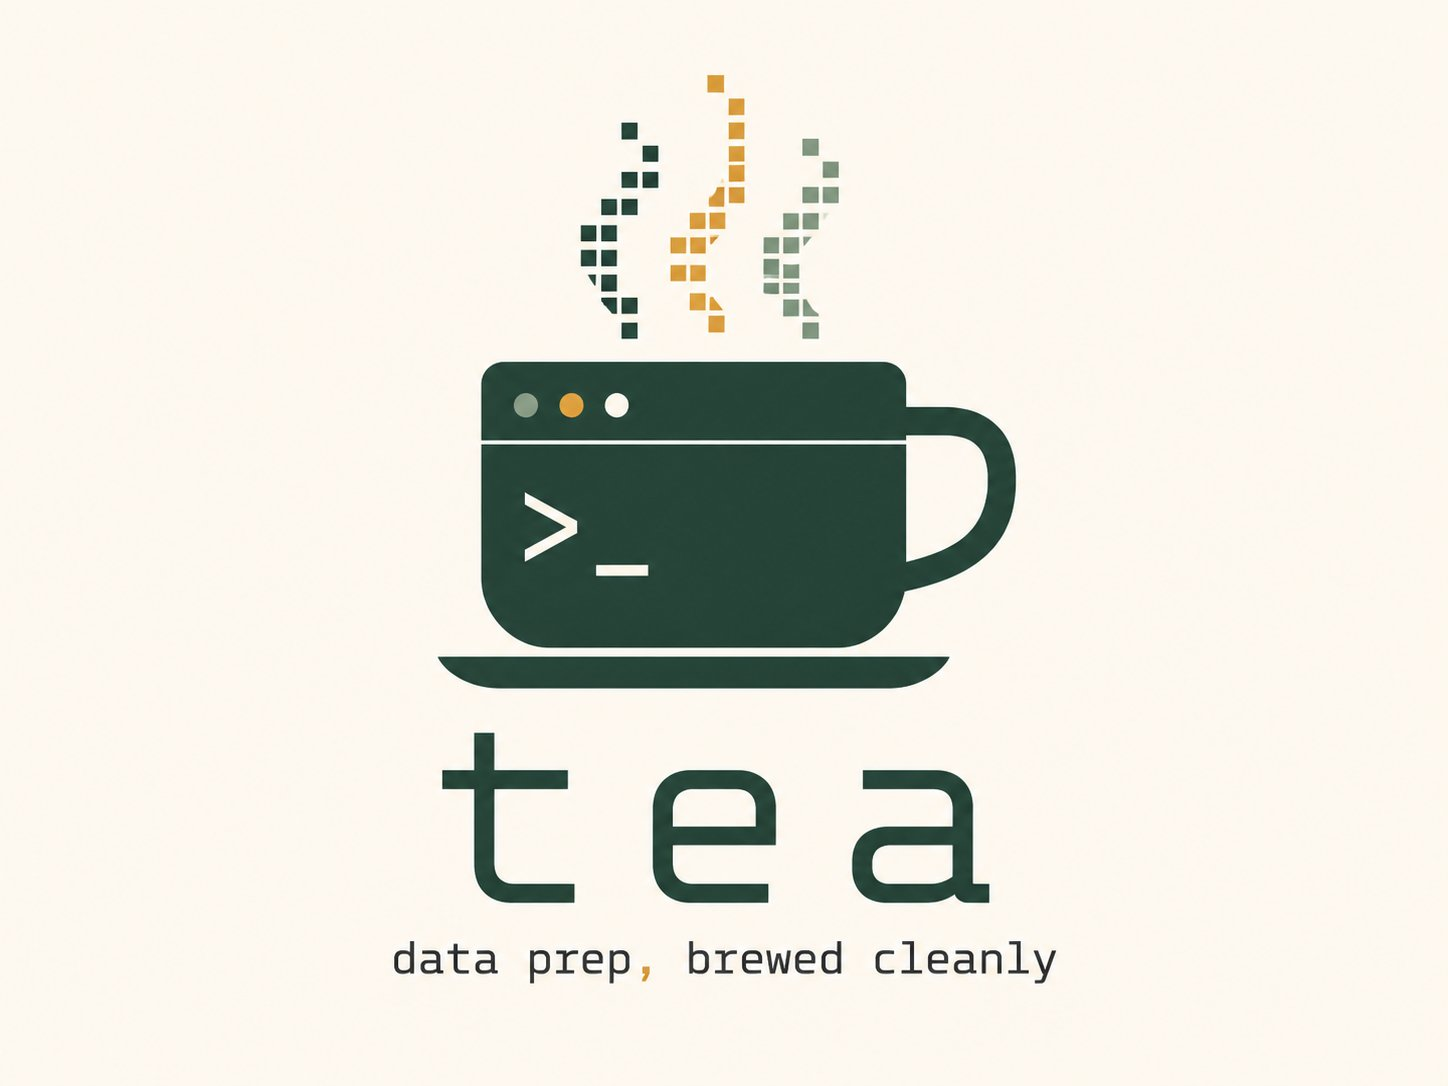
\includegraphics[width=0.55\textwidth]{tea_logo.jpg}\\[0.5em]
{\Huge\bfseries version \teaversion}\\[0.8em]
{\Large User guide and reference}\\[1.2em]
{\large Mico Mrkaic}\\[0.3em]
{\large \today}
\end{center}

\vspace{1.5em}
\begin{center}
\begin{minipage}{0.85\textwidth}
\small
\textbf{Abstract.} \texttt{tea} is a small command-line program for the
data-prep-to-quick-estimate loop economists use Stata for: import, clean,
generate variables, run regressions, panel methods, MLE, IV, and ARIMA ---
plus publication-grade SVG graphics and six bundled practice datasets,
including the complete IMF World Economic Outlook database.  The syntax
is close to Stata's where they overlap; the semantics are faithful where
it matters (missing-value algebra, the \texttt{by:} prefix, gap-aware
time-series operators, factor variables).  \texttt{tea} also runs entirely
in a web browser via WebAssembly, with no installation, and its output is
byte-identical across machines and numerical libraries.  This manual
covers installation, a guided tour, every command, the bundled data, and
escape hatches to Python/R for things \texttt{tea} does not handle.

\vspace{1em}
\textbf{Audience.}  Applied economists, policy analysts, and graduate
students familiar with Stata.  No Stata experience is strictly required,
but the manual assumes you know what \texttt{regress} is and what panel
data looks like.

\vspace{1em}
\textbf{Status.}  v\teaversion\ follows the v1.0 field-testing release.
It has passed 42 regression tests byte-identically on three configurations
(native gcc + OpenBLAS in release and sanitizer builds, and WebAssembly
clang + reference BLAS), is clean under AddressSanitizer and
UndefinedBehaviorSanitizer, and builds warning-free under
\texttt{-Wall -Wextra -Werror}.  Field testing continues; please report
what breaks.

\vspace{1em}
\textbf{AI-assisted development.}  This software was developed with the
assistance of an AI coding assistant (Anthropic's Claude).  The design
decisions, mathematical specifications, scope choices, and final
acceptance of each component were the author's; the AI contributed
substantial portions of the implementation, drafted regression tests,
and produced the first draft of this manual.  All code was reviewed
before inclusion.  This manual was likewise drafted with AI assistance
and edited by the author.  Bugs and design flaws are the author's
responsibility.

\vspace{1em}
\textbf{License.}  GPLv3 or later.  Copyright \textcopyright\ 2026
Mico Mrkaic.  See the \texttt{LICENSE} file in the distribution for
the full text.  \texttt{tea} is an independent open-source project,
not affiliated with or endorsed by StataCorp LLC.  The bundled datasets
retain their original licenses and citations; see the ``Bundled
datasets'' chapter and \texttt{data/SOURCES.md}.
\end{minipage}
\end{center}
\clearpage
